\documentclass[aspectratio=169]{beamer}

% Solarized Theme
\usecolortheme[light, accent=orange]{solarized}
\beamertemplatenavigationsymbolsempty

% Packages
\usepackage[T1]{fontenc}
\usepackage[utf8]{inputenc}
\usepackage[english]{babel}

\usepackage{graphicx}
\usepackage{rotating}
\usepackage{tikz}
\usepackage{tikzsymbols}
\usetikzlibrary{positioning, math, automata}
\setbeamersize{text margin left=-10pt,text margin right=-10pt}


\begin{document}

\begin{frame}
    \frametitle{
        \hspace{0.1cm} Michalis Panayides \hspace{0.6cm}
        \begin{minipage}{.15\textwidth}
            
\includegraphics[width=0.8\textwidth, trim={0, 0, 20, 0}, clip]{Bin/cyprus_flag.png}
        \end{minipage}
        \begin{minipage}{.15\textwidth}
            
\includegraphics[width=0.7\textwidth, trim={140 60 140 60}, clip]{Bin/welsh_flag.png}
        \end{minipage}
        \begin{minipage}{.09\textwidth}
            
\includegraphics[width=\textwidth]{Bin/uni_logo.png}        
        \end{minipage}
        \begin{minipage}{.2\textwidth}
            
\includegraphics[width=\textwidth]{Bin/THISLogo.png}
        \end{minipage}
    }
    
    \centering
    \begin{minipage}{.4\textwidth}
        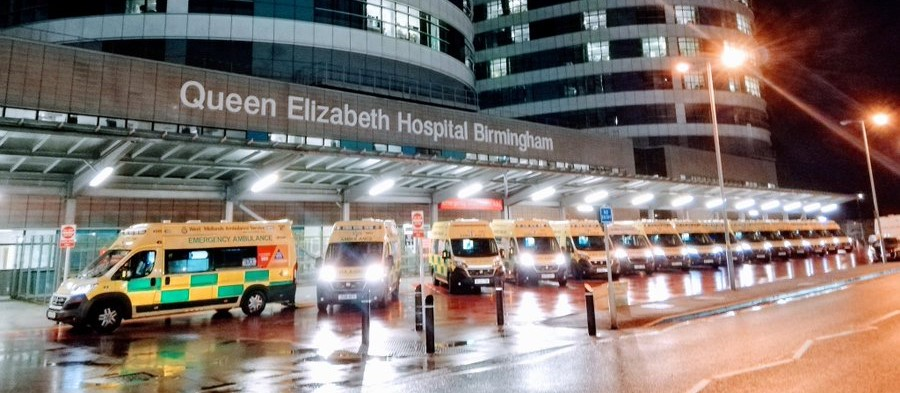
\includegraphics[width=\textwidth]{Bin/ambulance_queue.jpg}
    \end{minipage}
    \hspace{0.2cm}
    \begin{minipage}{.5\textwidth}
        \centering
        \begin{figure}
            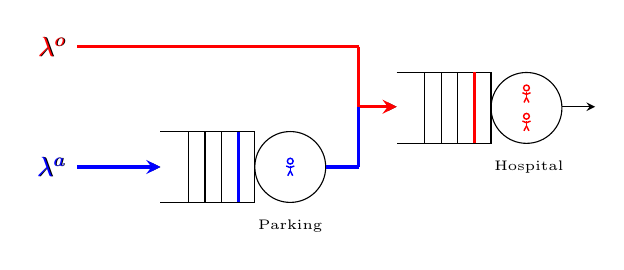
\begin{tikzpicture}[>=stealth, scale=0.6],
                % the rectangle with vertical rules (Queue 1)
                \draw (0,0) -- ++(2cm,0) -- ++(0,-1.5cm) -- ++(-2cm,0);
                \foreach \i in {1,...,4}
                \draw (2cm-\i*10pt,0) -- +(0,-1.5cm);
                
                % the circle (Queue 1)
                \draw (2.75,-0.75cm) circle [radius=0.75cm];
        
                % the rectangle with vertical rules (Queue 2)
                \draw (5,1.25) -- ++(2cm,0) -- ++(0,-1.5cm) -- ++(-2cm,0);
                \foreach \i in {1,...,4}
                \draw (7cm-\i*10pt,1.25) -- +(0,-1.5cm);
        
                % the circle (Queue 2)
                \draw (7.75,0.5) circle [radius=0.75cm];
        
                % the arrows and labels (Queue 1+2)
                \draw[->] (8.5,0.525) -- +(20pt,0);
                \node[align=center] at (1cm,-2cm) {};
                \node[align=center] at (2.75cm,-2cm) {\tiny{Parking}};
                \node[align=center] at (6cm,-0.75cm) {};
                \node[align=center] at (7.8cm,-0.75cm) {\tiny{Hospital}};
                
                % Ambulance lines
                \draw[<-] (0,-0.75) -- +(-50pt,0) node[left] {\( \lambda^a \)};
                \draw[-] (3.5,-0.75) -- +(20pt,0);
                \draw (4.2, 0.525) -- (4.2, -0.75);
    
                % Others lines
                \draw (4.2, 1.8) -- +(-169.5pt,0) node[left] {\( \lambda^o \)};
                \draw (4.2, 1.8) -- (4.2, 0.525);
                \draw[->] (4.2, 0.525) -- (5, 0.525);  
    
                % Animations
                \node[draw=none, red] at (7.75,0.8) {\Strichmaxerl[1]};
                \node[draw=none, red] at (7.75,0.2) {\Strichmaxerl[1]};
                \draw[red, very thick] (4.2, 1.8) -- +(-169.5pt,0) node[left] {\( \lambda^o \)};
                \draw[red, very thick] (4.2, 1.8) -- (4.2, 0.525);
                \draw[->, red, very thick] (4.2, 0.525) -- (5, 0.525);
                \draw[-, blue, very thick] (3.5,-0.75) -- +(20pt,0);
                \draw[blue, very thick] (4.2, 0.525) -- (4.2, -0.75);
                \draw[<-, blue, very thick] (0,-0.75) -- +(-50pt,0) node[left] {\( \lambda^a \)};
                \node[draw=none, blue] at (2.75,-0.75) {\Strichmaxerl[1]};
                \draw[blue, very thick] (2cm-10pt,0) -- +(0,-1.5cm);
                \draw[red, very thick] (7cm-10pt,1.25) -- +(0,-1.5cm);
            \end{tikzpicture}
            % \caption*{\scriptsize{Queueing Model}}
        \end{figure}
    \end{minipage}

    \vspace{0.01cm}

    \begin{minipage}{.47\textwidth}
        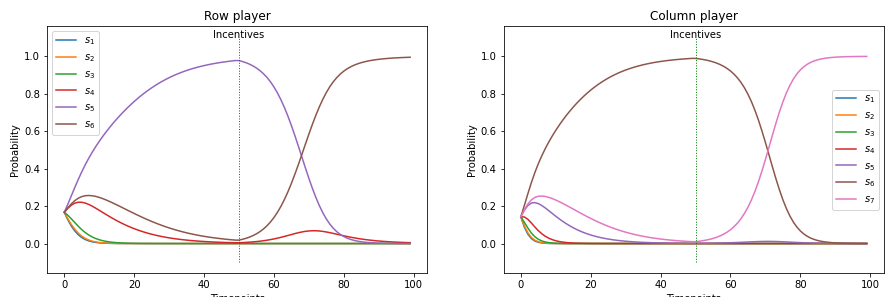
\includegraphics[width=.98\textwidth]{Bin/ARD_penalty_game.png}
    \end{minipage}
    \begin{minipage}{.47\textwidth}
        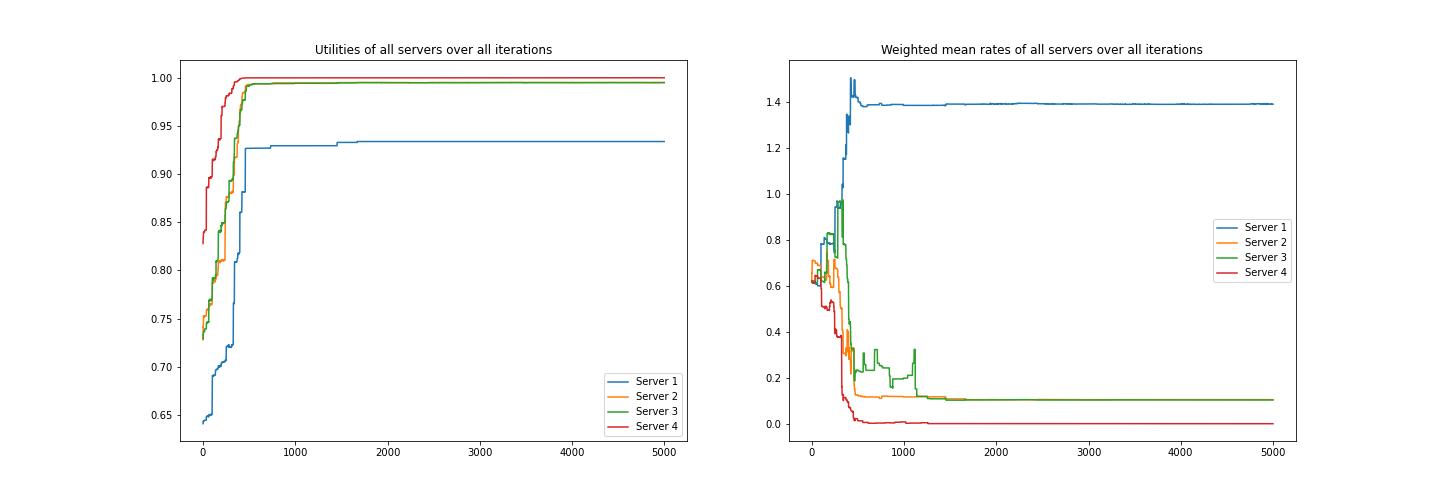
\includegraphics[width=.98\textwidth]{Bin/reinforcement_learning.png}
    \end{minipage}


\end{frame}


\end{document}